\documentclass[../../main.tex]{subfiles}
\graphicspath{{\subfix{../images/}}} % 指定图片目录,后续可以直接使用图片文件名。
\begin{document}

\section{简答题}
\begin{enumerate}
  \item \textbf{中心势场中的单粒子哈密顿量为 $\begin{aligned}
    H = \frac{\vec{p}^{2}}{2M} + V(r)
  \end{aligned}$. 轨道角动量 $\vec{L} = \vec{r}\times \vec{p}$, 那么 $[\vec{L},H] = ?$}
  
{\color{gray}{  由于是中心势场, 不妨设 $V(r) = r^{n}$, 则
  \begin{align*}
    [\vec{L},H] &= \left[\sum_{ijk}\epsilon_{ijk}\hat{x}_{i}x_{j}p_{k},\sum_{\alpha}^{3}\frac{p_{\alpha}^{2}}{2m}+r^{n}\right] = \frac{1}{2m}\sum_{ijk\alpha}\epsilon_{ijk}\hat{x}_{i}[x_{j}p_{k},p_{\alpha}^{2}] + \sum_{ijk}\epsilon_{ijk}\hat{x}_{i}[x_{j}p_{k},r^{n}]\\
    &= \frac{1}{2m}\sum_{ijk\alpha}\hat{x}_{i}\epsilon_{ijk}\left\{\cancel{x_{j}p_{\alpha}[p_{k},p_{\alpha}]} + \cancel{x_{j}[p_{k},p_{\alpha}]p_{\alpha}} + p_{\alpha}[x_{j},p_{\alpha}]p_{k} + [x_{j},p_{\alpha}]p_{\alpha}p_{k}\right\} + \sum_{ijk}\epsilon_{ijk}\hat{x}_{i}x_{j}[-i\hbar\frac{\partial}{\partial x_{k}},r^{n}]\\
    &= \frac{1}{2m}\sum_{ijk\alpha}2i\hbar\delta_{j\alpha}p_{\alpha}p_{k} + \sum_{ijk}\epsilon_{ijk}\hat{x}_{i}x_{j}\left(-i\hbar nr^{n-1} r^{-\frac{1}{2}}x_{k}\right)\\
    &= \sum_{ijk}\epsilon_{ijk}\hat{x}_{i}\left\{\frac{i\hbar}{m}p_{j}p_{k} + (-i\hbar nr^{n - \frac{3}{2}})x_{j}x_{k}\right\}
  \end{align*}
  注意到 $j\iff k$ 和 $\epsilon_{ijk}$ 的反对称性质, 可以得到 $[\vec{L},H] = \boxed{0}$.}}

  \item \textbf{考虑一阶近似, 当 $i\neq f$ 时, 跃迁概率为
  \begin{align*}
    P_{i\rightarrow f}(t) = \frac{1}{\hbar^{2}}\left|\int_{0}^{t}\mathrm{d}t^{\prime}\langle f|V(t^{\prime})|i\rangle e^{\mathrm{i}\omega_{fi}t^{\prime}}\right|^{2}
  \end{align*}
  其中 $\hbar\omega_{fi} = E_{f} - E_{i}$. 当微扰为
  \begin{align*}
    V(t) = \left\{\begin{aligned}
      V e^{-\mathrm{i}\omega t}\quad &t>0\\
      0\quad &t<0
    \end{aligned}\right.
  \end{align*}
  跃迁概率为?}

{\color{gray}{  \begin{align*}
    P_{i\rightarrow f}(t) &= \frac{1}{\hbar^{2}}\left|\left|\int_{0}^{t}\mathrm{d}t^{\prime}\langle f|Ve^{-\mathrm{i}\omega t^{\prime}}|i\rangle e^{\mathrm{i}\omega_{fi}t^{\prime}}\right|\right|^{2} 
    = \frac{1}{\hbar^{2}}\left|\left|\int_{0}^{t}\mathrm{d}t^{\prime}\langle f|V|i\rangle e^{-\mathrm{i}\omega t^{\prime}} e^{\mathrm{i}\omega_{fi}t^{\prime}}\right|\right|^{2}\\
    &=\frac{1}{\hbar^{2}}\left|\left|\int_{0}^{t}\mathrm{d}t^{\prime}\langle f|V|i\rangle  e^{\mathrm{i}(\omega_{fi}-\omega)t^{\prime}}\right|\right|^{2} = \frac{1}{\hbar^{2}}\left|\left|\int_{0}^{t}\mathrm{d}t^{\prime}\langle f|V|i\rangle  e^{\mathrm{i}\Delta\omega t^{\prime}}\right|\right|^{2}\\
    \left|\left|\int_{0}^{t}\mathrm{d}t^{\prime}e^{\mathrm{i}\Delta\omega t^{\prime}}\right|\right|^{2} &= \left|\left|\frac{e^{\mathrm{i}\Delta\omega t}-1}{\mathrm{i}\omega}\right|\right|^{2} = \frac{(e^{\mathrm{i}\Delta\omega t}-1)(e^{-\mathrm{i}\Delta\omega t}-1)}{(\Delta\omega)^{2}} = \frac{2-2\cos{\Delta t}}{(\Delta\omega)^{2}} = \frac{4}{(\Delta\omega)^{2}}\sin^{2}{\left(\frac{\Delta\omega t}{2}\right)}\\
    P_{i\rightarrow f}(t) &= \boxed{\frac{4\left|\langle f|V|i\rangle\right|^{2}}{\hbar^{2}(\Delta\omega)^{2}}\sin^{2}{\left(\frac{\Delta\omega t}{2}\right)}}
  \end{align*}}}

  \item \textbf{算符 $\begin{aligned}
    \Omega(t)\equiv U^{-1}(t)U_{0}(t)
  \end{aligned}$, 算符 $\begin{aligned}
    \Omega_{\pm}\equiv \lim_{t\rightarrow \mp\infty}\Omega(t)
  \end{aligned}$, 其中
  \begin{itemize}
    \item $U_{0}(t) = e^{-\mathrm{i}H_{0}t/\hbar}$ 是自由系统 $H_{0}$ 的时间演化算符;
    \item $\begin{aligned}
    U(t) = e^{-\mathrm{i}Ht/\hbar}
  \end{aligned}$ 是短程势散射系统的时间演化算符. 
  \end{itemize}
  $H = H_{0} + V$. 散射算符定义为 $S\equiv \Omega^{\dagger}_{-}\Omega_{+}$, 那么 $[S, H_{0}]=?$ }
  
  \item \textbf{动量空间中自由粒子的 Dirac 方程可以写为
  \begin{align*}
    \left(E - \vec{\sigma}\cdot\vec{p}\right)\chi_{+}(\vec{p}) &= m\chi_{-}(\vec{p})\\
    \left(E + \vec{\sigma}\cdot\vec{p}\right)\chi_{-}(\vec{p}) &= m\chi_{+}(\vec{p})
  \end{align*}
  当质量 $m=0$时, 两个 Weyl 旋量之间没有耦合, 得到动量空间中的 Weyl 方程
  \begin{align*}
    \left(E - \vec{\sigma}\cdot\vec{p}\right)\chi_{+} = 0, \quad \left(E + \vec{\sigma}\cdot\vec{p}\right)\chi_{-} = 0
  \end{align*}
  定义螺旋度算符为 $\begin{aligned}
    \frac{1}{2}\hat{\vec{p}}\cdot\vec{\sigma}
  \end{aligned}$, 其中 $\begin{aligned}
    \hat{\vec{p}} = \frac{\vec{p}}{|\vec{p}|}
  \end{aligned}$, 那么可知 Weyl 旋量 $\chi_{\pm}$ 恰好是螺旋度算符的本征态, 本征值分别为?}

  \item \textbf{一个可以制备 Bell 态的简单量子线路为}

  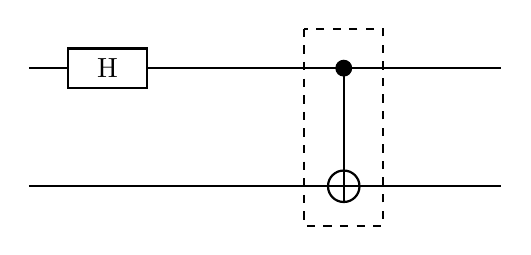
\begin{tikzpicture}

    % 绘制量子线路水平线
    \draw[thick] (0,0) -- (0.5,0); % 上线
    \draw[thick] (1.5,0) -- (6,0); % 上线
    \draw[thick] (0,-1.5) -- (6,-1.5); % 下线
    % 上线的H门
    \draw[thick] (0.5,-0.25) rectangle (1.5,0.25); 
    \node at (1,0) {H};
    % 上线的黑圆点
    \filldraw[black] (4,0) circle (0.1);
    % 下线的控制符号(十字)
    \draw[thick] (4,-1.5) circle (0.2); % 空心圆
    \draw[thick] (4,-1.7) -- (4,-1.4); % 垂直线
    \draw[thick] (3.8,-1.5) -- (4.2,-1.5); % 水平线
    % 连接黑圆点与十字
    \draw[thick] (4,0) -- (4,-1.5);
    % 绘制虚线框
    \draw[dashed,thick] (3.5,0.5) rectangle (4.5,-2);
    \end{tikzpicture}

  \textbf{它包含两个张量: 一个 Hadamard gate (H) 和一个 controlled NOT gate (CNOT)(虚线框里), 在 $S^{z}$ 表象下它们的矩阵表示为,
  \begin{align*}
    H = \frac{1}{\sqrt{2}}\begin{pmatrix}
      1 & 1\\
      1 & -1
    \end{pmatrix},\\
    \text{CNOT} = e^{\frac{\mathrm{i}\pi}{4}(\mathbb{I} - \sigma_{1}^{z})\otimes (\mathbb{I} - \sigma_{2}^{x})}
  \end{align*}
  将以上量子线路作用到 $|\uparrow\uparrow\rangle$ 上得到的态为?}
\end{enumerate}
\end{document}